\chapter{Implementation}
This chapter details the practical process of transforming the architectural blueprint from Chapter~3, ``System Design,'' into a functional simulation platform. The content covers the preparation of the host environment, the containerized build process for core components, and the orchestration of the entire distributed system using Docker Compose. The source code for this implementation are available on GitHub\footnote{\url{https://github.com/pandeng65536/Modern-Delay-Tolerant-Email/tree/main/Code}}.

\section{Environment and Dependency Preparation}

\subsection*{Host Environment and Core Software}
The simulation platform was developed and tested in the following environment:

\begin{itemize}
    \item Host Operating System: Ubuntu~24.04.2~LTS
    \item Container Engine: Docker~Engine v28.0.4
    \item Container Orchestration Tool: Docker~Compose v2.34.0
\end{itemize}

\subsection*{Compilation of Dependencies}
A key challenge during implementation was the version management of core dependency libraries. It was determined that the successful compilation and stable operation of BPMail required specific minimum versions of its dependencies, particularly \texttt{gmime}. However, the versions available in the official Ubuntu~24.04 software repositories were outdated and did not meet these requirements.

As direct installation via \texttt{apt-get} was not feasible, this dissertation adopted a strategy of manually compiling these dependencies from source. This was achieved by packaging the required source code versions with the project files and automating the compilation and installation process within the mail-server container's \texttt{Dockerfile}. The primary dependencies include:

\begin{itemize}
    \item mbedtls v2.28.8: A lightweight, open-source TLS/SSL stack providing cryptographic support for ION-DTN.
    \item gmime v3.2.15: A C library for parsing and creating MIME messages, fundamental to BPMail's email processing capabilities.
    \item c-ares v1.34.4: An asynchronous DNS request library used by network applications such as BPMail.
\end{itemize}

Although this approach increased the complexity of the build process, it offered two key advantages. First, it completely resolved all version compatibility issues, ensuring the stable operation of the BPMail application. Second, it provided complete and precise control over the software environment, significantly enhancing the reproducibility and reliability of the simulation platform, while also demonstrating the depth and thoroughness of this implementation.

\section{Containerized Implementation}
This section provides a detailed account of the build and configuration process for each independent component of the simulation platform.

\subsection{Mail Server Container}

The mail server container is the most complex component in this simulation, integrating three primary functions: email services (sending and receiving), a DTN node, and the email-DTN gateway.

\subsubsection*{Dockerfile Analysis}

The complete build process for this container is defined in \texttt{mail-server/Dockerfile}, which executes the following key stages:

\begin{enumerate}
    \item \textit{Base Environment}: The official \texttt{ubuntu:24.04} image is used as the base.
    \item \textit{Service Installation}: Using \texttt{apt-get} to install Postfix, Dovecot, and essential compilation and network debugging tools.
    \item \textit{Compilation of Dependencies}: As outlined previously, specific versions of \texttt{mbedtls}, \texttt{gmime}, and \texttt{c-ares} are required. The \texttt{COPY} directive is used to add their source code to the image, after which they are compiled and installed using their respective build systems (\texttt{make}, \texttt{./configure}, \texttt{cmake}).
    \item \textit{Compilation of the ION-DTN}: With \texttt{mbedtls} already in place, the ION-DTN stack is compiled. The process uses \texttt{autoreconf} to generate configuration scripts, followed by \texttt{./configure} with mbedtls support enabled (\texttt{--enable-crypto-mbedtls}), and finally \texttt{make \&\& make install}. Runtime configuration files for ION-DTN (e.g., the \texttt{.rc} files defining node EIDs and contact plans) were pre-configured and included with the source. This allows the startup script to simply run \texttt{ionstart} to load the correct configuration. The \texttt{ldconfig} command is used to ensure that newly installed shared libraries are discoverable.
    \item \textit{Compilation of the BPMail Gateway}: Once dependencies such as \texttt{gmime} and \texttt{c-ares} are ready, BPMail is compiled using the Meson build system.
    
    \begin{lstlisting}[language=bash,caption={Meson Build \& Install Stage}]
meson setup build
meson compile -C build
meson install -C build
    \end{lstlisting}

  This installs the gateway's core programs such as \texttt{bpmailsend}.
  \item \textit{Installation of Thunderbird Client}: For end-to-end debugging, Thunderbird is installed. Since Ubuntu~24.04 installs Thunderbird via Snap by default (problematic inside containers), a workaround is applied by adding the Mozilla PPA and forcing use of the traditional \texttt{.deb} package:

  \begin{lstlisting}[language=bash,caption={Install Thunderbird from Mozilla PPA}]
RUN add-apt-repository ppa:mozillateam/ppa
RUN cat <<EOF > /etc/apt/preferences.d/mozilla-ppa
Package: *
Pin: release o=LP-PPA-mozillateam
Pin-Priority: 1001
EOF
RUN apt-get update && apt-get install -y thunderbird
  \end{lstlisting}

\end{enumerate}

\subsubsection*{Entrypoint Execution}
After installation of all components, the container's \texttt{CMD} is set to run the entrypoint script \texttt{/mail-server.sh}.

\subsection*{Entrypoint Script (\texttt{mail-server.sh})}
This script is central to automated container configuration. On startup, it performs:

\begin{enumerate}
  \item \textit{Network Configuration}: Reads the environment variable \texttt{\$GATEWAY} from \texttt{docker-compose.yml} and sets it as the container's default gateway. This enables communication with the ``outside world'' (i.e., the delay node).
  \item \textit{Postfix and BPMail Integration}: Uses \texttt{\$HOSTNAME} to distinguish between \texttt{mail-1} and \texttt{mail-2}, applying different configurations accordingly.
  \begin{itemize}
    \item Appends a \texttt{pipe} transport service named \texttt{bp} to \texttt{master.cf}, which invokes \texttt{bpmailsend} for outgoing mail.
    \item Creates \texttt{/etc/postfix/transport} to map a destination domain to the \texttt{bp} service and specify the destination node's ION EID.
  \end{itemize}

  \begin{lstlisting}[language=bash,caption={Example snippet for \texttt{mail-1}}]
MASTER_CF="/etc/postfix/master.cf"
POSTFIX_TRANSPORT_FILE="/etc/postfix/transport"
if [[ "$HOSTNAME" == "mail-1" ]]; then
  echo "bp    unix  -    n     n     -     -     pipe" >> "$MASTER_CF"
  echo "  flags=ODR user=user argv=/usr/local/bin/bpmailsend -t 1 21 ${nexthop}" >> "$MASTER_CF"
  echo "mail-2.a.com   bp:ipn:3.129" >> "${POSTFIX_TRANSPORT_FILE}"
  postmap "${POSTFIX_TRANSPORT_FILE}"
fi
  \end{lstlisting}

  \item \textit{Dovecot Configuration}: Uses \texttt{sed} to adjust configuration files for the Maildir format and Postfix LMTP delivery.
  \item \textit{Service Startup}: Starts \texttt{postfix} and \texttt{dovecot}, then—based on \texttt{\$HOSTNAME}—launches the correct ION node and the BPMail receiving daemon (\texttt{bpmail2postfix.sh}), ensuring service dependencies are respected.
\end{enumerate}


\subsection{Network Delay Simulator Container}
This container, while simple in structure, serves a critical function. Its Dockerfile is based on \texttt{wbitt/network-multitool}, a public image rich with networking utilities, and is configured by copying and executing a startup script.

\subsubsection*{Network Delay Script (\texttt{delay-server.sh})}

This script executes upon container startup and is responsible for injecting network latency into the simulation platform:

\begin{lstlisting}[language=bash,caption={delay-server.sh startup script}]
#!/bin/bash
tc qdisc add dev eth0 root netem delay 1000ms
tc qdisc add dev eth1 root netem delay 1000ms
sysctl -w net.ipv4.ip_forward=1
tail -f /dev/null
\end{lstlisting}

The script uses the \texttt{tc qdisc} command to add a fixed 1000\,ms delay to the virtual network interfaces connecting to the ``Earth'' network (\texttt{eth0}) and the ``Moon'' network (\texttt{eth1}). It also enables IP forwarding via \texttt{sysctl}, allowing the container to function as a router between the two subnets.  
To simulate different network delays or disruptions in later experiments, only this script needs to be modified.

\subsection{User Client Containers}

In the \texttt{docker-compose.yml} file, the services named \texttt{client-1} and \texttt{client-2} function as the user terminals. Although they use the same base image as the mail servers, their configuration and purpose are different.

\subsubsection*{GUI Forwarding}

As shown in the following \texttt{docker-compose.yml} snippet, the container is configured to forward its GUI display to the host machine's desktop. This is achieved by setting Wayland-related environment variables and mounting the corresponding runtime directory as a volume, facilitating direct graphical interaction with the Thunderbird client.

\begin{lstlisting}[caption={docker-compose.yml: GUI forwarding for client-1}]
client-1:
  build: ./mail-server
  hostname: client-1
  environment:
    - MOZ_ENABLE_WAYLAND=1
    - WAYLAND_DISPLAY=${WAYLAND_DISPLAY}
    - XDG_RUNTIME_DIR=${XDG_RUNTIME_DIR}
  volumes:
    - ${XDG_RUNTIME_DIR}/${WAYLAND_DISPLAY}:${XDG_RUNTIME_DIR}/${WAYLAND_DISPLAY}:ro
  # ... other volumes ...
\end{lstlisting}

\subsubsection*{Thunderbird Configuration}
The Thunderbird profile was pre-configured on the host machine, and then mounted directly into the container's /root/.thunderbird directory upon startup. This approach obviated the need for tedious manual configuration each time the containers were launched.

The pre-configured profile contains all necessary settings (e.g., display name, email address and password) for the two user accounts, \texttt{user@mail-1.a.com} and \texttt{user@mail-2.a.com}, including saved security exceptions for the server certificates.

In this simulation environment, I use the default self-signed certificates generated by Postfix and Dovecot during installation. Consequently, when Thunderbird first connected to the server, it was unable to verify their identity, resulting in a security warning as shown in Figure \ref{fig:security_warning}. After manually accepting and saving the exception, a standard TLS/SSL encrypted channel is established. All subsequent communication between the client and servers is encrypted.
\begin{figure}[ht]
      \centering
      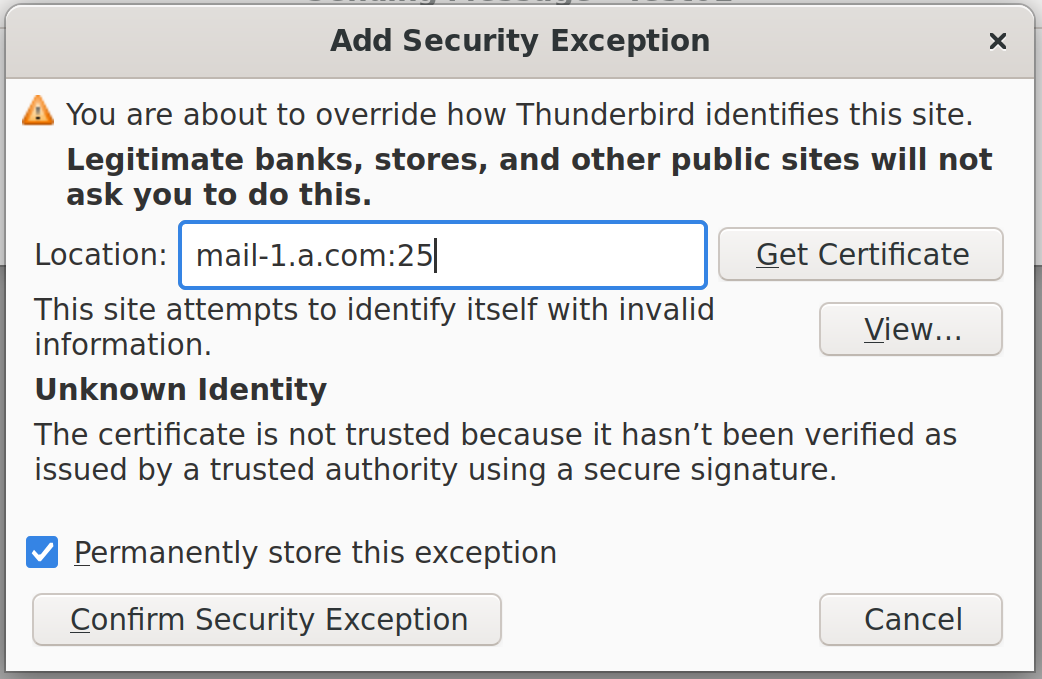
\includegraphics[width=0.8\textwidth]{Implementation/security_warning.png}
      \caption{Thunderbird security warning for self-signed certificate}
      \label{fig:security_warning}
\end{figure}

A similar certificate trust issue also exists in the server-to-server communication. Because the two Postfix instances each use their own self-signed certificate, they do not trust each other's identity during SMTP exchanges. Nevertheless, the SMTP connection between the two servers is still encrypted using TLS.

\section{System Orchestration and Startup}
The \texttt{docker-compose.yml} file acts as the master controller for the entire simulation platform, defining all components and their interconnections.

\subsection*{Service Definitions}
It defines the five core services: \texttt{delay-server}, \texttt{mail-1}, \texttt{mail-2}, \texttt{client-1}, and \texttt{client-2}.

Each service definition specifies its build context, hostname, static IP address, and necessary permissions (\texttt{cap\_add: [NET\_ADMIN]}).  
A key design element is the use of environment variables and the startup script to enforce cross-subnet traffic routing.  

The \texttt{GATEWAY} variable is injected into the \texttt{mail-1} and \texttt{mail-2} services, and the \texttt{mail-server.sh} script within each container reads this variable to dynamically set its default gateway to the IP address of the \texttt{delay-server}.  
Because the \texttt{delay-server} is the only node connected to both subnets, this design forces all inter-regional IP traffic to be routed through it, ensuring that the network impairments configured with \texttt{tc} are precisely applied to the critical communication link.


\subsection*{Network Definitions}
This section defines two independent bridge networks, \texttt{mail-1\_net} (Earth) and \texttt{mail-2\_net} (Moon), each with a distinct IP subnet.  
The service configurations in \texttt{docker-compose.yml} connect \texttt{mail-1} \& \texttt{client-1} to \texttt{mail-1\_net}, and \texttt{mail-2} \& \texttt{client-2} to \texttt{mail-2\_net}.  
The \texttt{delay-server} is uniquely connected to both networks, establishing it as the mandatory communication relay between Earth and Moon.  
This ensures that all inter-regional traffic traverses the \texttt{delay-server}, allowing the network impairments configured via \texttt{tc} to be precisely applied to the critical communication link.

\begin{lstlisting}[caption={docker-compose.yml: network definitions}]
networks:
  mail-1_net:
    driver: bridge
    ipam:
      driver: default
      config:
        - subnet: 172.21.0.0/24
  mail-2_net:
    driver: bridge
    ipam:
      driver: default
      config:
        - subnet: 172.22.0.0/24
\end{lstlisting}

\subsection*{System Startup}
The startup process is divided into two phases: deploying the background services and launching the foreground client.

\subsubsection*{System StartupBuild and Start Background Services}
First, all background services (\texttt{mail-1}, \texttt{mail-2}, \texttt{delay-server}) and the client container ``shell'' are built and launched in detached mode using a single command.  
The \texttt{--build} flag ensures that the images are rebuilt from the latest \texttt{Dockerfile} prior to launch:

\begin{lstlisting}[language=bash,caption={Building and launching background services}]
docker compose up -d --build
\end{lstlisting}

\paragraph{Launch the Graphical Mail Client}
After the backend services are running, the graphical Thunderbird client is launched manually.  
First, the host machine's X server must be authorized to accept connections from the container.  
Then, a shell is opened inside the running client container (\texttt{client-1}):

\begin{lstlisting}[language=bash,caption={Authorizing X server and opening client container shell}]
# Allow clients to connect to the local X server
xhost +
# Execute a shell inside the running client container
docker compose exec client-1 /bin/bash
\end{lstlisting}

From within the container's shell, the Thunderbird application is started:

\begin{lstlisting}[language=bash,caption={Launching Thunderbird inside the container}]
# Launch the Thunderbird program inside the container
thunderbird
\end{lstlisting}


Thanks to the pre-configured GUI forwarding and the mounted profile volume, the graphical Thunderbird interface appears on the host's desktop with all email accounts ready for immediate use.

\section{Summary}
This chapter has provided a detailed account of the practical process of transforming the design blueprint into a working reality. By combining Dockerfiles for component encapsulation, shell scripts for automated configuration, and Docker Compose for system orchestration, a complex, multi-component distributed system was successfully converted into an automated, one-click simulation platform. Key implementation details, from the compilation of third-party dependencies from source to the deep integration of Postfix with BPMail and the precise control of the network environment, have been clearly articulated. At this point, a fully functional and highly controllable experimental environment has been deployed, setting a solid foundation for the system testing and limitation analysis in the next chapter.
